\graphicspath{ {mainmatter/Marquez-Borbon_2015/} }

\title*{2015: Fourteen Years of NIME: The Value and Meaning of `Community' in Interactive Music Research}
\titlerunning{`Community' in Interactive Music Research}

\author{Adnan Marquez-Borbon and Paul Stapleton}
\authorrunning{Marquez-Borbon and Stapleton}

%\institute{Adnan Marquez-Borbon \at Sonic Arts Research Centre, Queen's University Belfast, Belfast, Northern Ireland, \email{a.marquez-borbon@qub.ac.uk}
%\and Paul Stapleton \at Sonic Arts Research Centre, Queen's University Belfast, Belfast, Northern Ireland, \email{p.stapleton@qub.ac.uk}
%}
%
%
\maketitle

\abstract*{This paper examines the notion of community as commonly employed within NIME discourses. Our aim is to clarify and define the term through the community of practice framework. We argue that through its formal use and application, the notion of community becomes a significant space for the examination of emergent musical practices that could otherwise be overlooked. This paper defines community of practice, as originally developed in the social sciences by Lave and Wenger, and applies it within the NIME context through the examination of existing communities of practice such as the laptop performance community, laptop orchestras, as well as the Satellite CCRMA and Patchblocks communities.}

\section{Introduction}
In the 14 years of NIME's existence, the conference has showcased work of a highly varied nature produced in increasingly diverse contexts. Across these various practices, NIME has focused on developing novel or alternative musical interactions by merging together the principles, traditions and innovations from both Human-Computer Interaction and from 20th century Western European concert and experimental musics. Despite the desire for novelty driving these technological developments, this work is not realized within a vacuum and inherits, intentionally or not, characteristics of the social, cultural or economic environment from which it emerges. In effect, outcomes are still bound to theoretical and aesthetic influences from traditional musical practices regardless of the ebb and flow of fashionable research approaches and aims or performance styles and technologies. Transplanting these devices into established musical practices, or generating new ones, raises many questions that cannot be simply addressed by investigating isolated features of the devices themselves or through individual, isolated, developments of practice. 

%Motivation, purpose and main idea of paper
One recent approach that has gained greater interest within NIME research is the community aspect surrounding specific digital musical interactions. By taking a global perspective and moving away from the individual, it is expected that a shared knowledge and experience amongst the individuals within a group can yield both novel and lasting musical practices with a particular system. While the term community is often used, it is rarely defined or contextualized in NIME research by means of existing frameworks from other research disciplines, such as social sciences. In this light, the examined community is identified by default as part of a participatory design framework or in some cases loosely defined as an aggregation of practitioners, whether performers, designers or composers \cite{Gaye:2006,McPherson:2012,Vallis:2011}.

Indeed, it is our belief that new research in this area benefits from this perspective by delineating and examining the internal dynamics of communities surrounding digital musical interaction practices. However, due to a lack of supporting theoretical concepts, it can be easy to overlook important issues given the inability to examine the complexities of a community as they develop a mutually supported activity. Opportunities for examining different activities, such as teaching, learning and the development of new practices are potentially neglected \cite{Bowman:2009}.  Such behaviours may contribute in important ways to furthering our understanding of novel interactions and developing new musical practices within this domain. Attempting to find alternatives to the term community, rather than redefine and deepen it, may not be an entirely fruitful endeavour. As observed by Shelemay \cite{Shelemay:2011}, a rethinking of the concept may see the transmission of musical knowledge and performance not as `expressions or symbols of a given social grouping, but as an integral part of processes that can at different moments help generate, shape, and sustain new collectivities.' Given this position, in this paper we introduce and describe the community of practice and community of interest frameworks by presenting existing communities within NIME as case studies identified and examined through their learning activities. 

\section{Background}
While the notion of community in this domain is often used as a descriptor for an aggregate of people involved in activities relating to digital musical interaction design, in this section such groups will be analytically framed within the context of a community of practice in order to gain an understanding of how learning is supported.

\subsection{Learning in Context: Situated Learning and Communities of Practice}
Learning is an activity commonly thought of as occurring within a classroom environment and with an authority figure such as a teacher or instructor. This further taking place within a formal institution, or school, which determines specific curriculum, evaluation criteria and other educational protocols in order to evaluate the knowledge or competence of the pupil. Additionally, this learning context can be further framed through the specific pedagogical methods that are employed. However, this type of \textit{formal learning} is often criticised due to their abstracting, or separating, between the contents of learning (i.e. knowledge) and the actual practice in which these contents are applied. In other words, the school learning environment is seen as existing apart from the broader socio-cultural context in which we actually dwell in. 

The classroom education perspective is challenged by a number of models---such as situated learning and communities of practice---that attempt to remedy the problems of formal learning, as well as provide alternative learning scenarios. The situated learning framework \cite{Brown:1989,Lave:1991} asserts that knowledge is inextricably a product of the activity and situations in which it is produced. More than simply being \textit{situated} in time or space, situated learning implies that activity is \textit{in} and \textit{with} the world \cite{Lave:1991}. Situated learning, as a broad framework, offers different perspectives on how learning is carried out, whether as guided participation \cite{Rogoff:1995}, cognitive apprenticeship \cite{Brown:1989}, or legitimate peripheral participation (LPP) \cite{Lave:1991}. Despite their differences there is a consensus which views and describes learning in terms of activity and participation within a community of practice \cite{Rambusch:2005}. As originally defined by Lave and Wenger \cite[p.~98]{Lave:1991}, a community of practice (CoP) is `a set of relations among persons, activity, and world, over time and in relation with other tangential and overlapping communities of practice.' For Wenger in particular, a community of practice is more than a group of people who share a common interest or activity; it is a social structure that reflects shared histories of learning \cite{Wenger:1998}. For a more detailed comparison between different CoP definitions refer to Cox \cite{Cox:2005}.

Situated learning requires the engagement of the individual in `authentic' practice (i.e., activities of a domain framed by its culture) developing within a socio-cultural environment \cite{Brown:1989}. More than gaining abstract knowledge, learning requires actually engaging in the particular activities of a community. Gaining an understanding and mastery of knowledge and skill in this context requires learners to participate in such activities and let themselves be absorbed by the `culture of practice' \cite{Lave:1991}. Thus this process of establishing membership within a community is how an individual acquires knowledge and skills. This process of learning is defined by Lave and Wenger as legitimate peripheral participation (LPP) \cite{Lave:1991}. Although this concept emerged from the learning process observed in `traditional' apprenticeships (such as tailors or midwives), Lave and Wenger note that learning can occur in the absence of a formally organised apprenticeship or teacher. One of situated learning's most resonant critiques is that it obscures the process in which the individual transforms socio-cultural processes into mental processes. Lave and Wenger would refute such a premise since the claim itself divorces and abstracts mental and bodily activity (i.e., knowing-through-practice) from the social environment in which they are embedded. Nonetheless, Billett puts forth a model based in what he deems a complementarity between cognitive psychology and socio-cultural theory \cite{Billett:1996}. Billet's model suggests that higher-order procedural knowledge in the form of goal-directed problem-solving activities is used for generating and organising knowledge from specific and socially determined problems. Outcomes and their meanings are then regulated according to different experiences of the individual and the community. Similar approaches examining the social regulation of higher mental processes are presented in \cite{Arievitch:2005} and \cite{Rambusch:2006}.   


\section{NIME as a Community}
Recalling Lave and Wenger's original definition of a community of practice, as emergent from legitimate peripheral participation, we see that this particular model does not quite fit what is observed in the NIME community. Namely, there is no form of learning analogous to apprenticeships (in the strict traditional sense), where learning involves the gradual participation of the novice in the communal practices and activities. Without a doubt there are expert and novice practitioners within NIME; however, the learning that occurs is mainly institutionalised and conducted through a teaching curriculum \cite{Fels:2009}. As distinguished by Lave and Wenger, a `teaching curriculum' is structured for newcomers and mediated by an instructor; it supplies boundaries and learning resources, and establishes the meaning of what is learned. This differs from a `learning curriculum' in that knowledge is explicitly taught and decontextualised from the socio-cultural environment in which the activity takes place \cite{Lave:1991}. Of course, attempting to educate through an apprenticeship model in modern academic settings is indeed impractical, hence the choice of applying structured pedagogical strategies. Nonetheless, as shown in the music domain, informal learning environments within communities of practice have proved successful in improving students' learning of performance, improvisation and composition skills, as well as enriching their own personal learning experiences \cite{MacMillan:2007,Waldron:2008,Waldron:2009}.

In the broadest organisational sense, NIME aims towards the goal of developing a shared body of work on new musical interface design. In this manner both joint enterprise and shared repertoire are met. Additionally, the NIME conference provides opportunities for developing personal networks, sharing experiences and learning from other members. Therefore the mutual engagement condition is satisfied. Given this view, NIME likely fits the community of practice profile. However, the community is not homogeneous; members do not engage in similar work in a particular domain. Practitioners from different domains---HCI, computer science, electrical engineering, (computer) music, and arts---engage in a joint enterprise. Perhaps NIME could appropriately be described as a `community-of-communities' \cite{Brown:1991}. This particular configuration is defined by Fischer as a \textit{community of interest} (CoI) \cite{Fischer:2009}. A CoI, in contrast to a CoP, attempts to solve a common task across multiple domains. In this manner, the overarching goal of NIME is to develop a body of work related to new digital instruments from different disciplines and perspectives (Table~\ref{Marquez-Borbon:fig:CoI}). 


\begin{table}[t]
\centering
\ra{1.2}
\caption{Differentiating CoP and CoI (from \cite{Fischer:2009})}
\label{Marquez-Borbon:fig:CoI}
\vspace{3pt} \noindent
\begin{tabular}{p{0.20\textwidth}p{0.4\textwidth}p{0.4\textwidth}}
\toprule
\textbf{Dimensions}     & \textbf{CoPs} & \textbf{CoIs} \\
\midrule  
Nature of Problems  	& Different tasks in the same domains 	& Common task across multiple domains \\
Knowledge development 	& Refinement of one knowledge systems; new ideas coming from within the practice & Synthesis and mutual learning through the integration of multiple knowledge systems \\
Major objectives 		& Codified knowledge, domain coverage 	& Shared understanding, making all voices heard \\ 
Weaknesses 				& Group-think 							& Lack of a shared understanding \\
Strengths				& Shared ontologies						& Social creativity; diversity; making all voices heard \\
People 					& Beginners and experts; apprentices and masters  & Stakeholders (owners of problems) from different domains \\
Learning 				& Legitimate peripheral participation 	& Informed participation \\
\bottomrule
\end{tabular}
\end{table}

% Modified to table
%
%\begin{figure}[t]
%	\centering
%		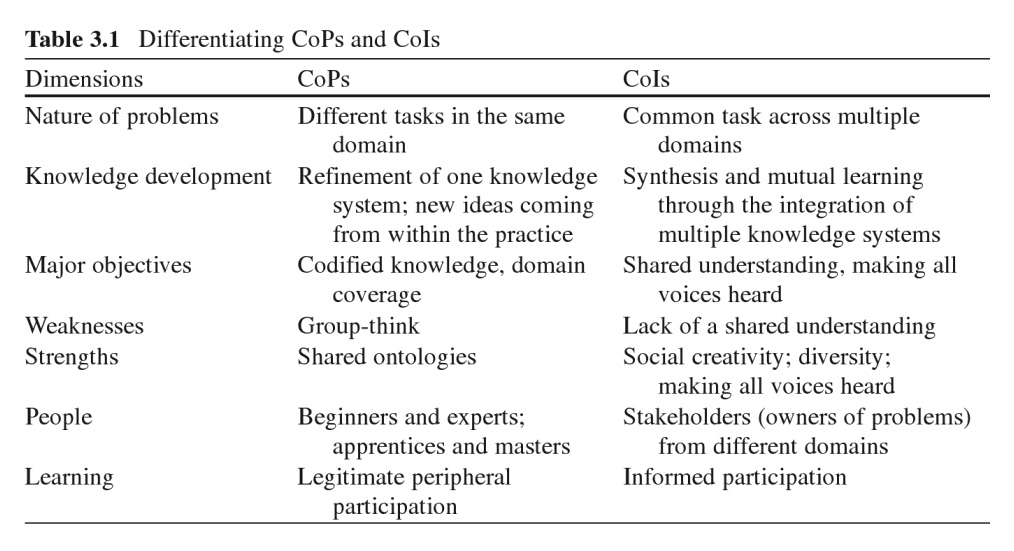
\includegraphics[width=1\columnwidth]{Fischer_2009_ch3_coi.jpg}
%	\caption{Differentiating CoP and CoI (from Fischer 2009)}
%	\label{Marquez-Borbon:fig:CoI}
%\end{figure}

The interdisciplinary nature of NIME can be deemed an asset. Indeed, Fischer observes that stakeholder diversity becomes a strength for this type of community. This same diversity, however, also produces a significant challenge due to a lack of shared understanding. Perspectives and vocabulary may initially differ, hence producing difficulties in communication \cite{Fischer:2009}. With time this understanding evolves incrementally, through collaborations producing ideas and external artefacts. Thus, there is a process of integration of multiple knowledge systems manifested in the form of synthesis and mutual learning. Learning in these communities, rather than through apprenticeship, is by `informed participation' which is characterised by the concurrency of experts and novices \cite{Fischer:2009}. Although it may seem contradictory, Fischer explains that expertise occurs when stakeholders communicate their knowledge to others; these same stakeholders become novices themselves when they learn from others who are experts in areas outside their own expertise.  

Specifically, discussions surrounding learning and pedagogy within this domain have centred on learning a diverse set of related topics ranging from music theory, composition, interaction design, and HCI to computer science, electrical engineering, and signal processing \cite{Cook:2009,DArcangelo:2002,Fels:2009,Leeuw:2012,Magnusson:2009a}. However, despite a few claims to the development of performance skills with new instruments \cite{Leeuw:2012}, there is a lack of supporting learning structures aside from prescribing prolonged practice or actual performance \cite{Butler:2008,Oore:2005,Zbyszynski:2008}. Competency in this domain, thus, is achieved by the mere accumulation of knowledge and its application in designs, whereas approaches for developing skilled performance are notoriously absent. The multiple reasons affecting this issue are discussed in depth by O'Modhrain \cite{OModhrain:2011}. However, inspecting specific practices within the broader community may shed light on the existence of such learning structures. 

\begin{figure}[t]
	\centering
		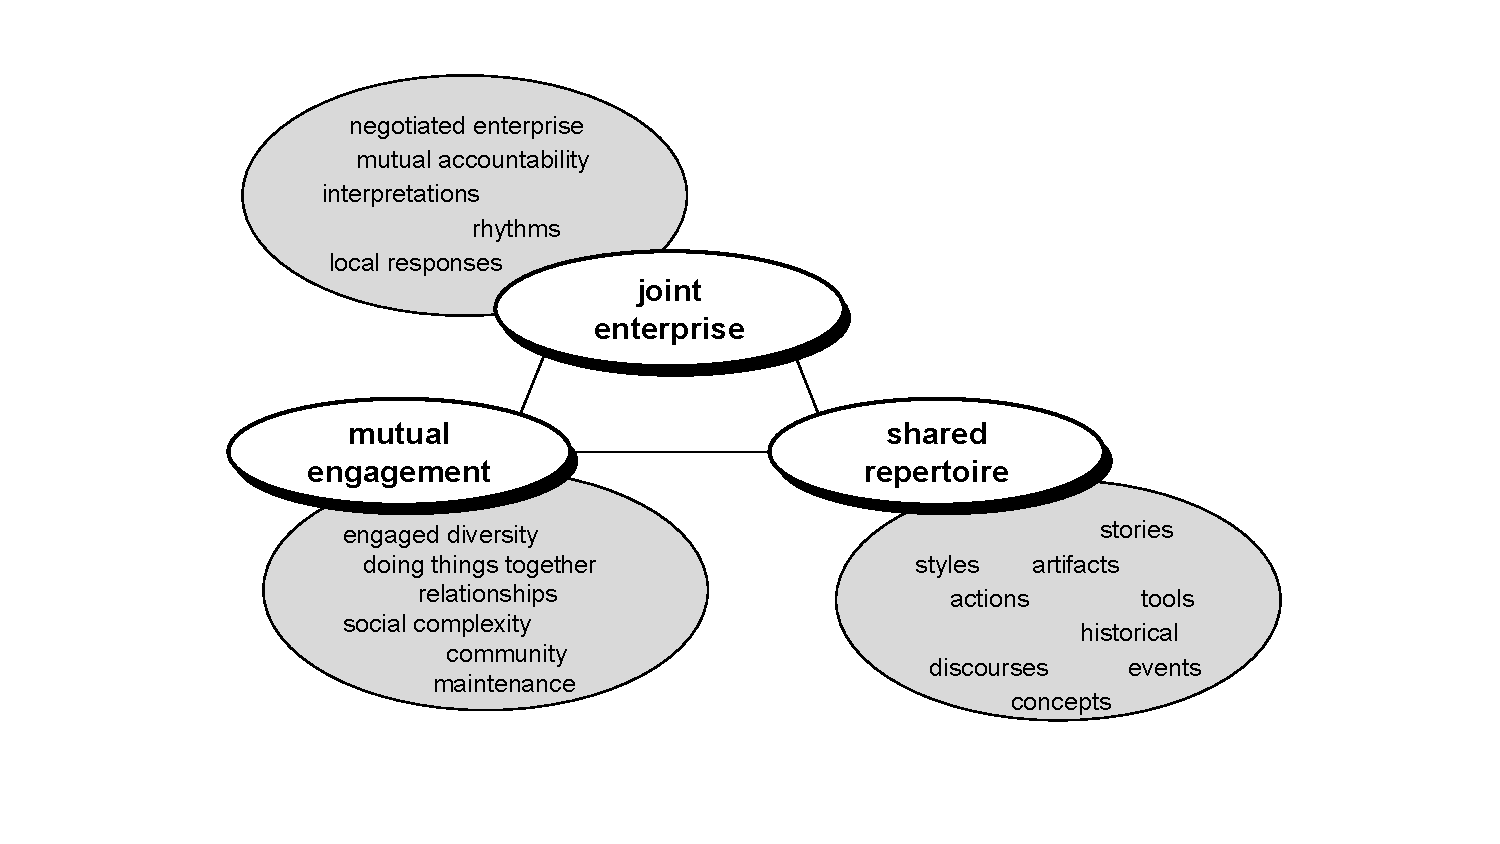
\includegraphics[width=1\columnwidth]{Wenger_1998_CoP.pdf}
	\caption{Dimensions of practice as the property of a community, within CoP (from Wegner 1998)}
	\label{Marquez-Borbon:fig:CoP}
\end{figure}


\subsection{Case Studies: Interactive Music Communities within NIME}
Emerging from electronic and computer music in general we can identify a number of communities that engage in ways that are distinguishable as being communities of practice. Some of these lie outside and overlap with NIME and academic institutions as seen in the Max/MSP, Pure Data, Super Collider, ChucK, monome \cite{Vallis:2011}, or even the circuit bending communities. However, in this discussion we will solely focus on those communities that have closely developed and established themselves alongside the institutional boundaries of the NIME ecology.  

Applying Wenger's later framework (Figure~\ref{Marquez-Borbon:fig:CoP}) within the broader NIME community, we can find smaller subsets that meet the criteria of a community of practice---a community based on the existing conditions of joint enterprise, mutual engagement and shared repertoire. The laptop performance community, as oriented towards performance and learning, meets such conditions. The laptop as a musical instrument has enjoyed a significant degree of longevity and gained a considerable amount of practitioners since the laptop became an increasingly affordable commodity in the 1990s. Despite the sustained criticisms of laptop performance \cite{Ostertag:2002,Richards:2008,Schloss:2003,Stuart:2003}, the laptop-as-instrument \cite{Magnusson:2010} has engendered a variety of practices involving a diversity of software tools, techniques, aesthetics, politics \cite{Grossmann:2008,Monroe:2003,Stuart:2003,Turner:2003}, as well as its own `genre' \cite{Cascone:2003}. This uptake has certainly benefited from the role of the Internet as a space supporting learning, interaction, and collaboration with other practitioners \cite{Cascone:2000}. Online forums and message boards permit obtaining relevant information, engaging in dialogue, and acquiring the appropriate software tools \cite{Cascone:2000}. In this manner, there is both a shared repertoire of practice-directed objects and a virtual space supporting opportunities for mutual engagement. 

More recently, laptop performance in academic contexts has gone through a process of formalisation in which performance practices have given rise to the `live coding' (Figure~\ref{Marquez-Borbon:fig:livecoding}) \cite{Collins:2003,Collins:2011,Magnusson:2011,Wang:2004,Ward:2004} and the `laptop orchestra' (Figure~\ref{Marquez-Borbon:fig:lork}) movements \cite{Fiebrink:2007,Trueman:2007,Wang:2008a}. The sub-communities of live coding and laptop orchestras can be deemed proper CoPs. Following Wenger's community elements, these communities have properly developed conditions for mutual engagement in which members, through participation, establish relationships of learning and collaboration in a joint enterprise (i.e., designing and performing music with laptop based instruments). 

\begin{figure}[t]
	\centering
		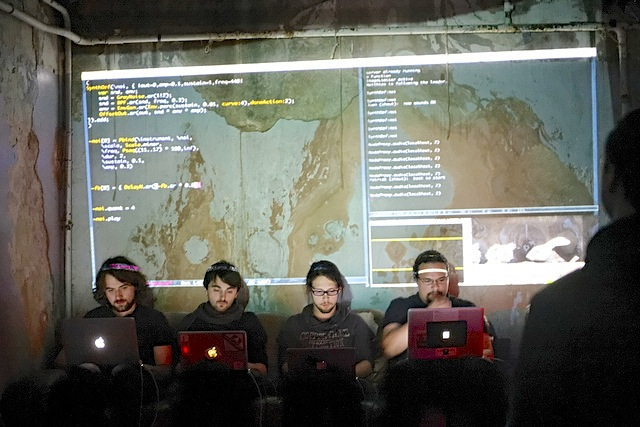
\includegraphics[width=9cm]{livecoding.jpg}
	\caption{Live Coding: Benoit and the Mandelbrots (Steve Welburn, CC-BY-SA)}
	\label{Marquez-Borbon:fig:livecoding}
\end{figure}

\begin{figure}[t]
	\centering
		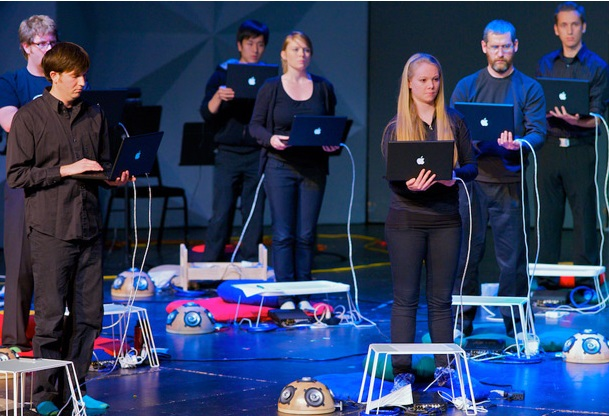
\includegraphics[width=9cm]{slork.jpg}
	\caption{Laptop Orchestra}
	\label{Marquez-Borbon:fig:lork}
\end{figure}

For both live coders and laptop orchestras the activity of performance is not the only goal. While performance is certainly important, the community itself has established other goals. This is apparent in the efforts for improving live coding languages and software, as well as documenting their practices, activities and other relevant information for distribution. In this manner, the structure of practice is not externally imposed, but is (re)negotiated by the members of the community; they themselves give meaning to actions, objects, and other elements important to the community itself. Similarly, values for judging performances are generated from within the community of practitioners \cite{Collins:2003,Magnusson:2011}. 

A shared repertoire emerges with time in the form of specific activities, symbols, or artefacts that show a history of mutual engagement. Whether they are expressed through laptop `battles,' established laptop-orchestra rehearsal routines and pieces \cite{Albert:2012}, or repositories of code and documentation \cite{Vallis:2011}, they show the development of the community and demonstrate how meaning changes over time. Of course, as Wenger \cite{Wenger:1998} comments, this meaning retains some degree of ambiguity. However, this ambiguity provides the basis for creating new practices. Despite the usage of online resources for communication and storage of materials, geographical location is not a strict condition for the establishment of a community of practice \cite{Waldron:2009,Wenger:1998}. Indeed, one can see that on some live-coding sites (for example, the Supercollider, Max/MSP or ChucK forums), levels of engagement and exchange are rather high \cite{Magnusson:2011}.     

Another recent and emergent community of practice in this context is the Satellite CCRMA community\footnote{\url{https://ccrma.stanford.edu/~eberdahl/Satellite/}} (Figure~\ref{Marquez-Borbon:fig:satellite}) \cite{Berdahl:2011}. In the few years of existence, Satellite CCRMA has gained traction as a compelling resource for developing embedded music computing applications. It has a well documented repository of information, as well as an active online community forum.\footnote{\url{https://groups.google.com/forum/\#!forum/satelliteccrma}} While the homepage is an important source of information for getting started with the platform, the forum plays a significant role in furthering the knowledge of members of the community. The forum provides an important source of information for continuing the development of one's practice. It is evident in the form of technical issues brought up during the deployment of the platform and implementation of more specific features. Forum members, aside from the webmaster, openly contribute their experiences and knowledge in order to solve common issues or prevent future problems. Additionally, members share their work with others as exemplars of the diverse technical capacities and artistic possibilities with the platform.

\begin{figure}[t]
	\centering
		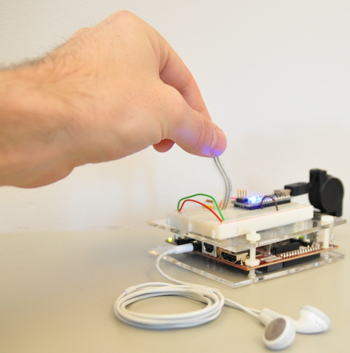
\includegraphics[width=9cm]{sat1.jpg}
	\caption{Satellite CCRMA}
	\label{Marquez-Borbon:fig:satellite}
\end{figure}

Our final example is Patchblocks\footnote{\url{http://patchblocks.com/}}, a tangible interface for collaborative performance (Figure~\ref{Marquez-Borbon:fig:patchblocks}). What is particularly interesting in this case is the fact that the notion of community as a resource for technological development was explicit since its inception \cite{Heinz:2010}. Such social factors are integrated in this tangible interface are through individual creation and the adaptation and sharing within a community which leads to the collaborative development of the interfaces' technology. Recently, the project has established a significant online community with a large and active user base invested in the development of both Patchblocks software and hardware. Patchblocks provides a striking contrast to other digital musical interaction projects where the community aspect is secondary to the projects' objectives and often emerges in a secondary or unintended fashion. Similarly, the notion of collaboration within Patchblocks is not limited to performance, but to the communal development of knowledge and technological resources. From these conditions it is evident that this particular project fits the CoP framework in an exemplary manner.  

\begin{figure}[t]
	\centering
		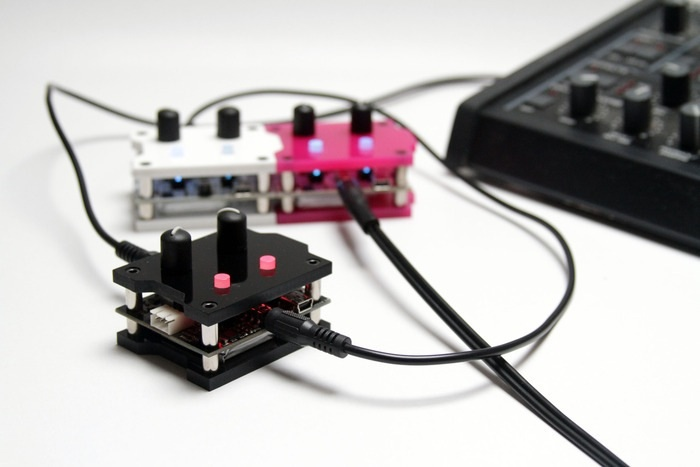
\includegraphics[width=9cm]{Patchblocks.jpg}
	\caption{Patchblocks}
	\label{Marquez-Borbon:fig:patchblocks}
\end{figure}


\section{Summary}
As presented in this paper, the notion of community in NIME is examined through the lens of a community of practice so as to identify its constituting elements and relationships amongst the members of existing communities as they learn through the development of a mutual activity. These communities of practice, as represented by live coding, laptop orchestra, Satellite CCRMA, and Patchblocks user groups, exemplify how learning diverse elements of digital musical interactions emerge and are structured in informal contexts. Through websites and forums, novices are introduced to the practices, tools, and human resources of the community in order to gain the necessary knowledge for embarking on their projects, as well as improving their competencies. The documented activities of the community serve to make public the activities and share the experiences of more skilled practitioners, thus structuring and guiding beginners own practice and learning. In this manner, novices are made aware of the specific criteria for achieving proficiency along with loosely established goals to attain. 

In examining the learning practices within a subset of communities we can note the presence of established mechanisms for judging what could be considered a `good' performance. This is particularly evident within the laptop performance and live coding communities. However, the absence of such mechanisms within the broader NIME community leads us to raise the questions of how can we develop a communal understanding of performance and how can we arrive to it, if it is possible to do so. Indeed, there is much to learn from the presented case studies as they may provide some answers to such complex questions (other lines of inquiry regarding judging NIME performances are presented in \cite{Gurevich:2009}). As it stands, the lack of a community understanding of performance inhibits the development of constructive critique which in turn inhibits forward movement.  

The community of practice framework is a powerful analytical resource for investigating the dynamic relationships and learning activities within social organizations. Although the presented case studies may provide an initial step towards understanding---through their actions, relationships, and outcomes---the complexities of a community, we firmly believe that such analytical tools can yield profound insights, as well as foster the development of new musical practices with digital musical interactions.


\section*{Author Commentary: Moving Forward---Notes on Participation, Diversity and Social Mediation in the NIME Community}
\paragraph{Adnan Marquez-Borbon and Paul Stapleton}

The ``community of practice framework'' outlined in our paper is one of many lenses available to better understand the value and meaning of community in the context of NIME. Regardless of the specific methods employed, NIME (as a conference and as a maturing community of interest) is now at the stage where it must urgently reflect on its motivations, values and future priorities. As a ``community-of-communities,'' NIME's mix of disciplines, methodologies, outputs and proclaimed openness to diversity has been widely celebrated. It is clear that the diverse and ad hoc nature of NIME has provided an effective starting point for bringing together cross-disciplinary expertise around the necessarily interdisciplinary field of interactive music technologies. However, the lack of coherent vision and critical reflection across NIME's various interest groups acts to marginalize or exclude individuals and collectives whose practices are not already supported by dominant social norms. Not all actors in NIME are speaking from the same position of power, and an openness to diversity does not automatically result in other voices being heard.

The need for a broadening of focus beyond questions such as design implementation to include ``questions of power, authority, legitimacy, participation, and intelligibility'' \cite{Irani:2010} is exemplified by an increase in reference to philosophy of technology, critical theory and social aesthetics at NIME's parent Conference on Human Factors in Computing Systems (CHI). We argue that both NIME and CHI have much to gain from a more widespread adoption of ``aesthetic and cultural reasoning'' \cite{Bardzell:2009}, particularly if our aim is to foster an inclusive community that more accurately reflects the growing diversity of social practices which adopt and adapt technologies for creative and political ends. 

Recent attempts to raise the visibility of marginalized groups within NIME [e.g. \cite{Born:2015}] have resulted in conversations which begin to productively address the power dynamics at play in our broader community.  Although it is clear that NIME is mediated by wider social inequalities (e.g. gender, ethnicity and class), it is likewise mediated by institutional structures that privilege different methods of knowing and doing. The decreasing representation of practice-based research in the NIME literature, in place of ``technical and scientific reporting,'' has been recently documented by Gurevich \cite{Gurevich:2015}. He further argues that the current tension between these research paradigms is unnecessary, yet remains inevitable without clearer explication of ``what could constitute legitimacy within the PBR community,'' and how this contingent and heterogeneous approach might ``interface'' with the more established and generalizable principles and methods of science.  Similarly, Green \cite{Green:2015} argues that practice-led research can be ``complementary to quantitative, controlled-condition methods'' by augmenting the ``generality of observation'' found in these methods ``in order to contend with musical practice in local, socially entangled, contentious and noisy complexity.'' Green laments that, despite the great potential NIME offers for a productive interdisciplinary convergence, NIME attempts to engage with music performance with little recognition of the ``wider issues'' of performance practice.

For us, it is clear that performance is the biggest casualty caused by a lack of rigorous critical reflection and communication across different areas of the NIME community. While new musical interfaces, systems or sensing devices are performed with each year, those from past conferences are at best recalled through anecdotes or as paper citations. Very few technological developments survive outside of NIME, or even within NIME over time. We suspect the primary cause is a lack of connection to sustained and emerging real world performance practices, and a lack of engagement with academic and professional communities that sustain these practices. The ``N'' in NIME itself is perhaps partially to blame, in that it resists the long-term development of performance pedagogies, repertoire and critical discourse necessary for the legitimisation of a performance community within the wider NIME community. It is noteworthy that NIME's self-proclaimed continual quest for novelty aligns with larger institution prioritises that privilege innovation and impact over actual content and substance.

Finally, if the musics produced by and through the innovations of our NIME community are to have wider artistic legitimacy, we must actively expand our genealogy beyond the canon of the European and American avant-garde. As Green \cite{Green:2015} has well argued, NIME could facilitate a move towards ``a pluralist aesthetic of electronic musicking'' through more formal reflection on, and ``sharing of,'' the diverse musical practices that inform and motivate our research.

\section*{Expert Commentary: NIME---A Community of Communities}
\paragraph{Michael J. Lyons}

I am not sure when I first heard the phrase \lq the NIME community.\rq The current community mailing list\footnote{community@nime.org}, named in 2007, might suggest NIME has consciously considered itself as a community for nearly a decade. However, I have the impression that only in recent years has NIME been frequently described as a community, both verbally and in articles published at the conference. 

The current article, the most recent in this collection, was selected because it is the first to explicitly attempt to analyze aspects of the NIME community. The authors base their approach on the theoretical frameworks of \lq situated learning\rq (SL) and \lq communities of practice\rq (CoP), which have long enjoyed broad influence in fields related to the sociology of learning, knowledge, and innovation. It is helpful to read this article in conjunction with key articles on SL and CoPs, and I can particularly recommend the lucid and insightful work of Brown and Duguid \cite{Brown:1989, Brown:1991}.

The article is therefore not really a survey of the NIME community, as the title might lead one to think, but an investigation of the NIME community from the viewpoint of a specific theoretical framework. Nonetheless, this offers readers  with some experience at NIME a valuable opportunity to reflect on the social processes at work in the community from a perspective they might not normally adopt.

To shorten the story, based on a taxonomy from the CoP literature, the authors conclude that the NIME community is not itself a CoP---it is too heterogeneous in approach. Rather, NIME more closely resembles a \lq community of interest\rq (CoI), in that it aims broadly to ``develop a body of work related to new digital instruments from different disciplines and perspectives.'' Admirably, the authors do not attempt to force-fit NIME into the CoP framework, writing instead that:

\begin{quotation}
Practitioners from different domains---HCI, computer science, electrical engineering, (computer) music, and arts---engage in a joint enterprise. Perhaps NIME could appropriately be described as a \lq community-of-communities.\rq
\end{quotation}

This corresponds closely with my view: multi-disciplinarity was an important aspect of the NIME workshop proposal \cite{Poupyrev:2001a} and has continued as an outstanding feature of the conference \cite{Lyons:2015}, which remains unusually open, for an academically oriented conference, to a plurality of approaches, tastes, and levels of expertise in both music and technology.

The authors locate bona-fide CoPs in several sub-communities affiliated with NIME. Their treatment is valuable and should serve as a basis for interesting further work, but this also falls short of being a survey: there are many such specialized groups, these have often evolved quite rapidly, sometimes spawning independent events. Moreover, this fragmented approach does not really shed much light on the community as a whole, and this leads me to ask: what other approaches could provide insight into the NIME community? 

Besides a theoretical critique, it would be revealing to attempt empirical work. Scientometric analyses of the NIME published proceedings, such as Jensenius' analysis \cite{Jensenius:2014} of gesture-related terminology, can also provide insight into aspects of the community. On a larger scale, Liu and co-workers \cite{Liu:2014} presented a detailed, fascinating empirically-based account of the CHI research community using co-word analysis. This not only maps the network of research interests of the community, but highlights the connectivity of interests and how these have changed over time. It should be possible to conduct a similar analysis of the NIME archive and this would serve to map and track the evolution of the activities and interests of the community.

Scientometrics does not directly address every sociological question and other complementary approaches, such as ethnography should also be valuable. Rigorous ethnographic studies, however, such as underlie CoP theory itself, demand a significant long-term commitment of resources and effort and may well face special challenges in the context of the shape-shifting field of new music technology. More closely knit sub-CoPs, such as the examples given in the current article, should be more amenable to ethnographic work, but we should take care that a reductionist approach does not lead us to ignore the ecology of the larger community.

A more modest proposal, for starters, is to survey NIMErs themselves about their experience of the community in which they participate, via interviews, questionnaires, and/or free reflection. This could leverage existing resources such as the conference mailing list, web portal, and other existing channels. Designed intelligently and positively, this would serve as a participatory, awareness-raising, and constructive community-building activity.
